\section{Benchmarking}
\label{sec:res_bench}
This section presents the result from the IOZone benchmarking tests run on each filesystem. The output result is divided into a table for each test for each filesystem. Each table presents the benchmark performance of the test for each file size and each buffer size. It is a table of five rows and 13 columns, where each cell is the performance of the test with the specific file size and buffer size. The complete data tables and graphs presenting the performance of each file system for the different file sizes can be found in Appendix~\ref{app:bench_data}.

Combining all the data in one table, we get the overall performance of a test. Using this data, we can plot a box plot presenting the spread of the values in the table. Figure~\ref{fig:res_box_ffs} presents a box plot of the benchmarking results of FFS.
% TODO: Fill in when have real data about ffs

\begin{figure}[!htb]
	\label{fig:res_box_ffs}
	\begin{center}
		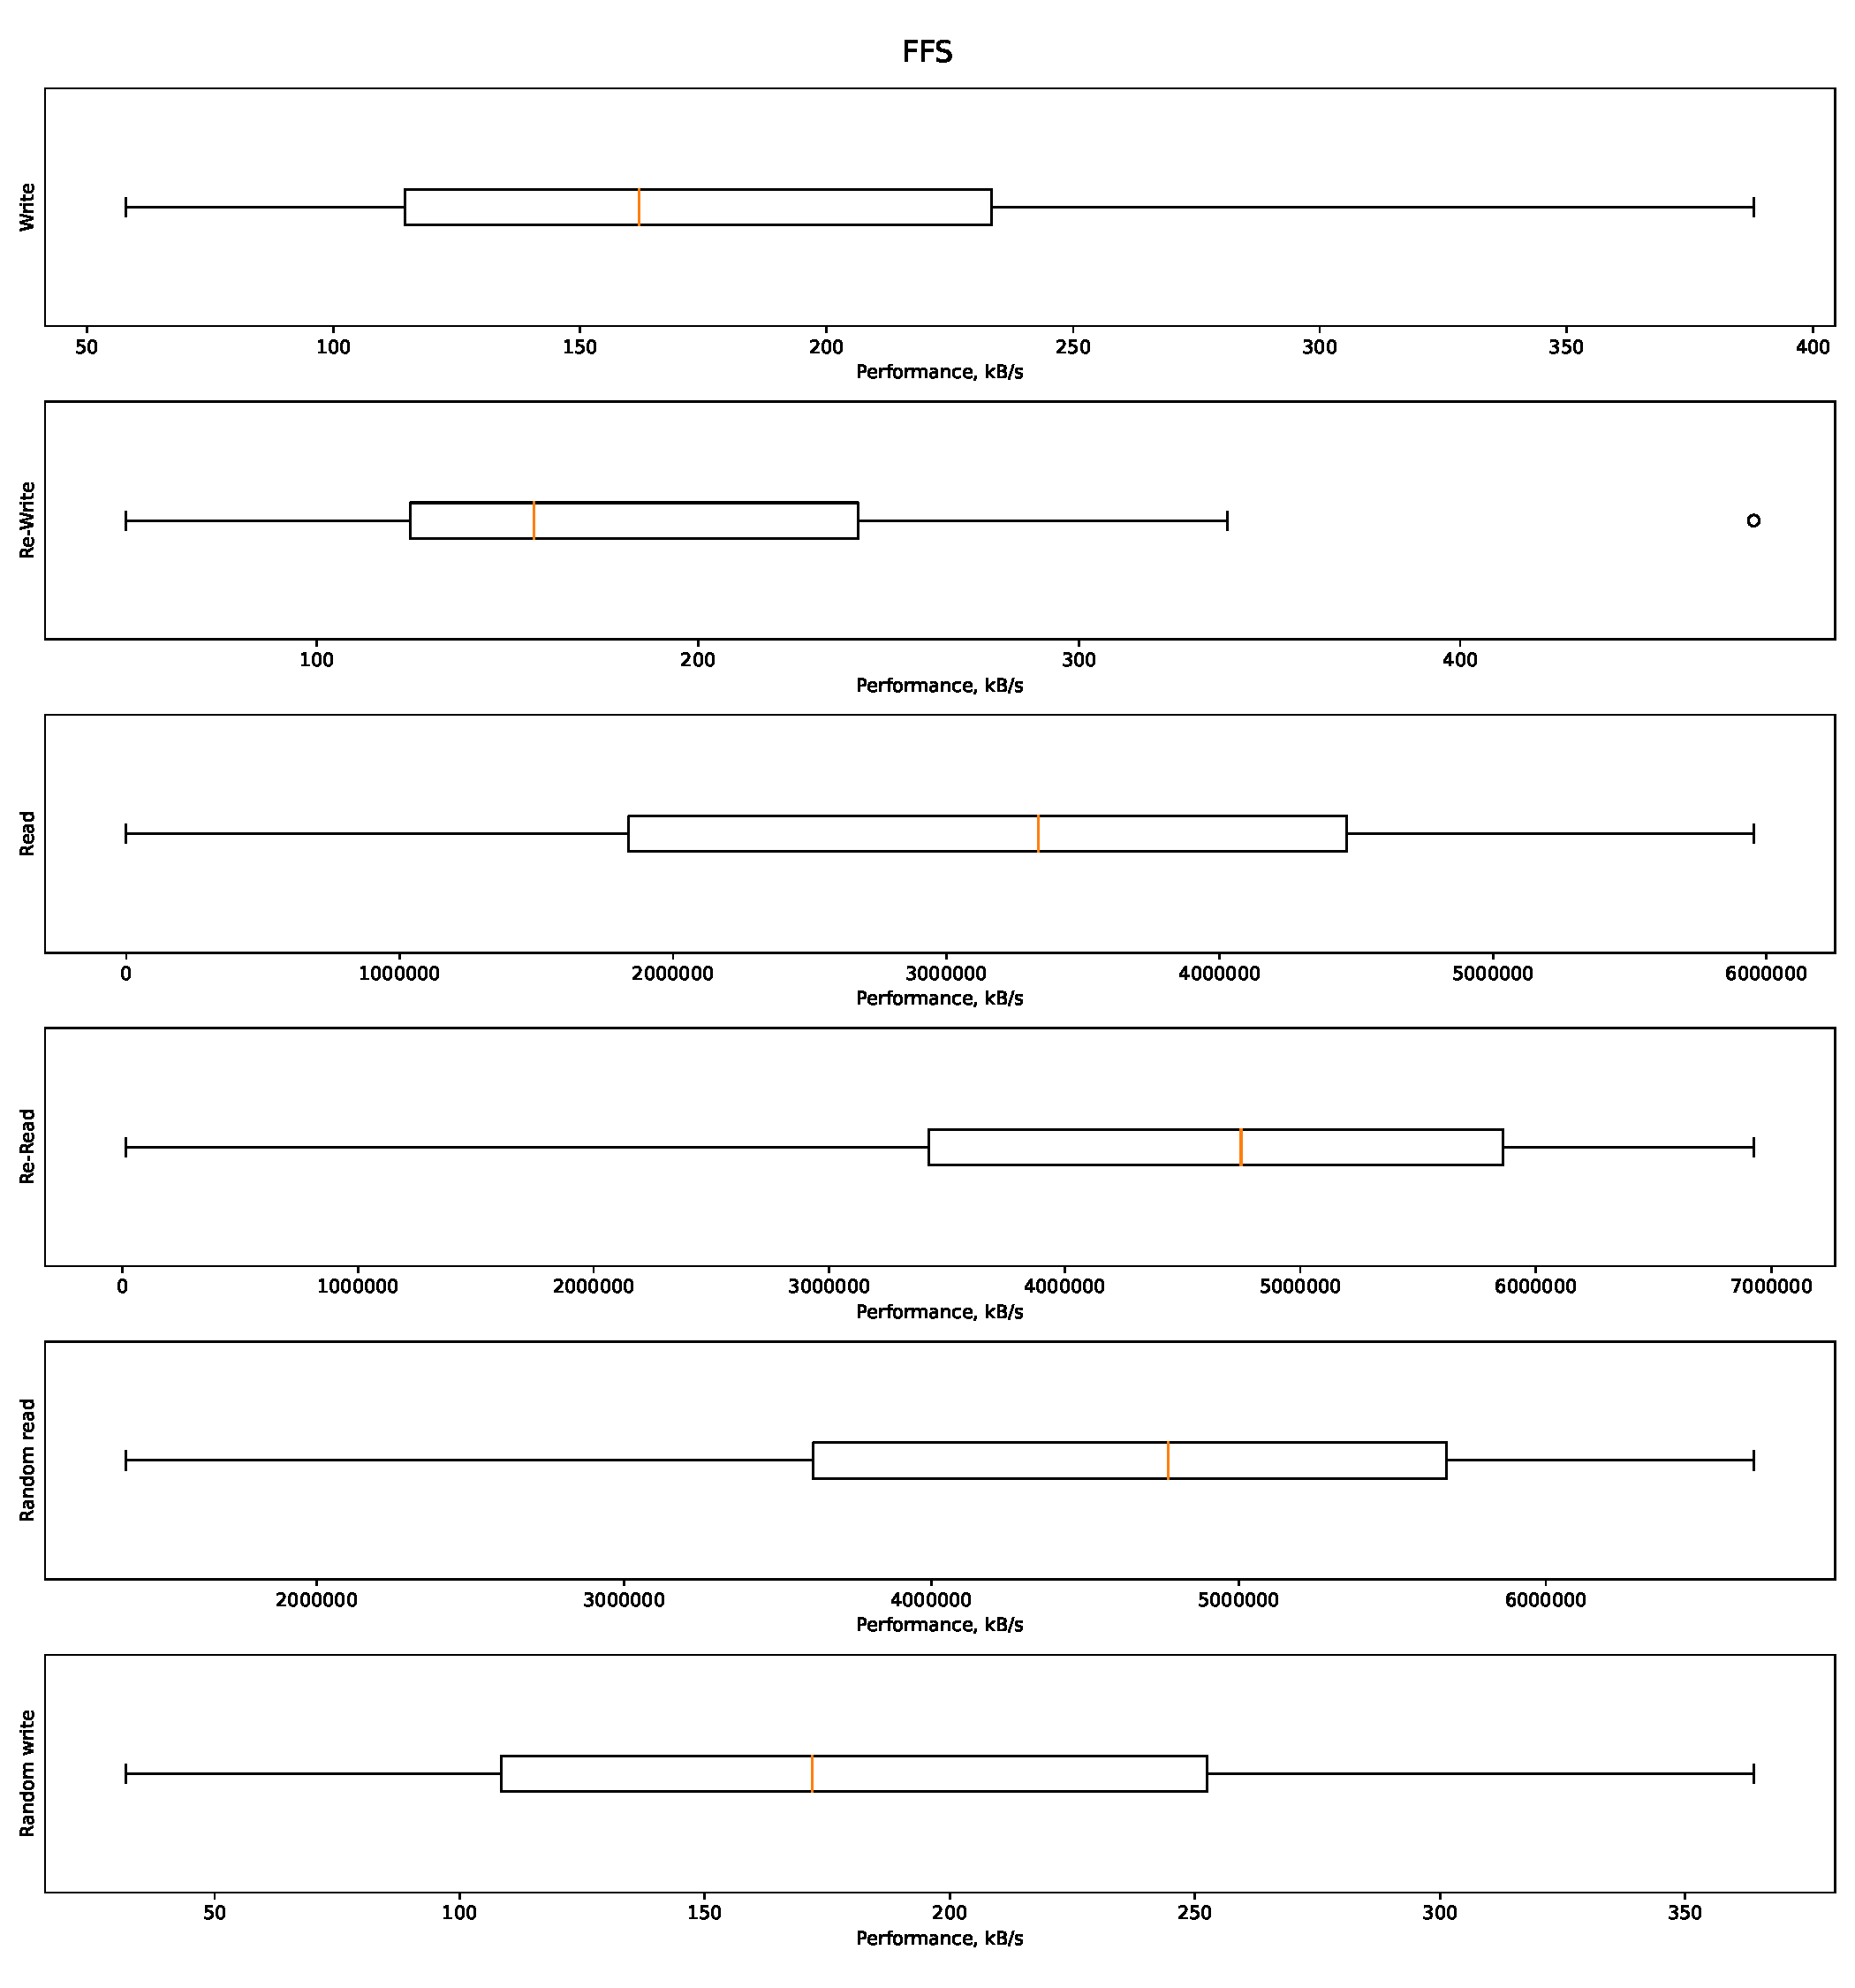
\includegraphics[width=1.0\textwidth]{figures/benchmarking/ffs/FFS-box.pdf}
	\end{center}
	\caption{Box plot of the IOZone output for the different tests for FFS}
\end{figure}


\begin{figure}[!htb]
	\label{fig:res_box_gcsf}
	\begin{center}
		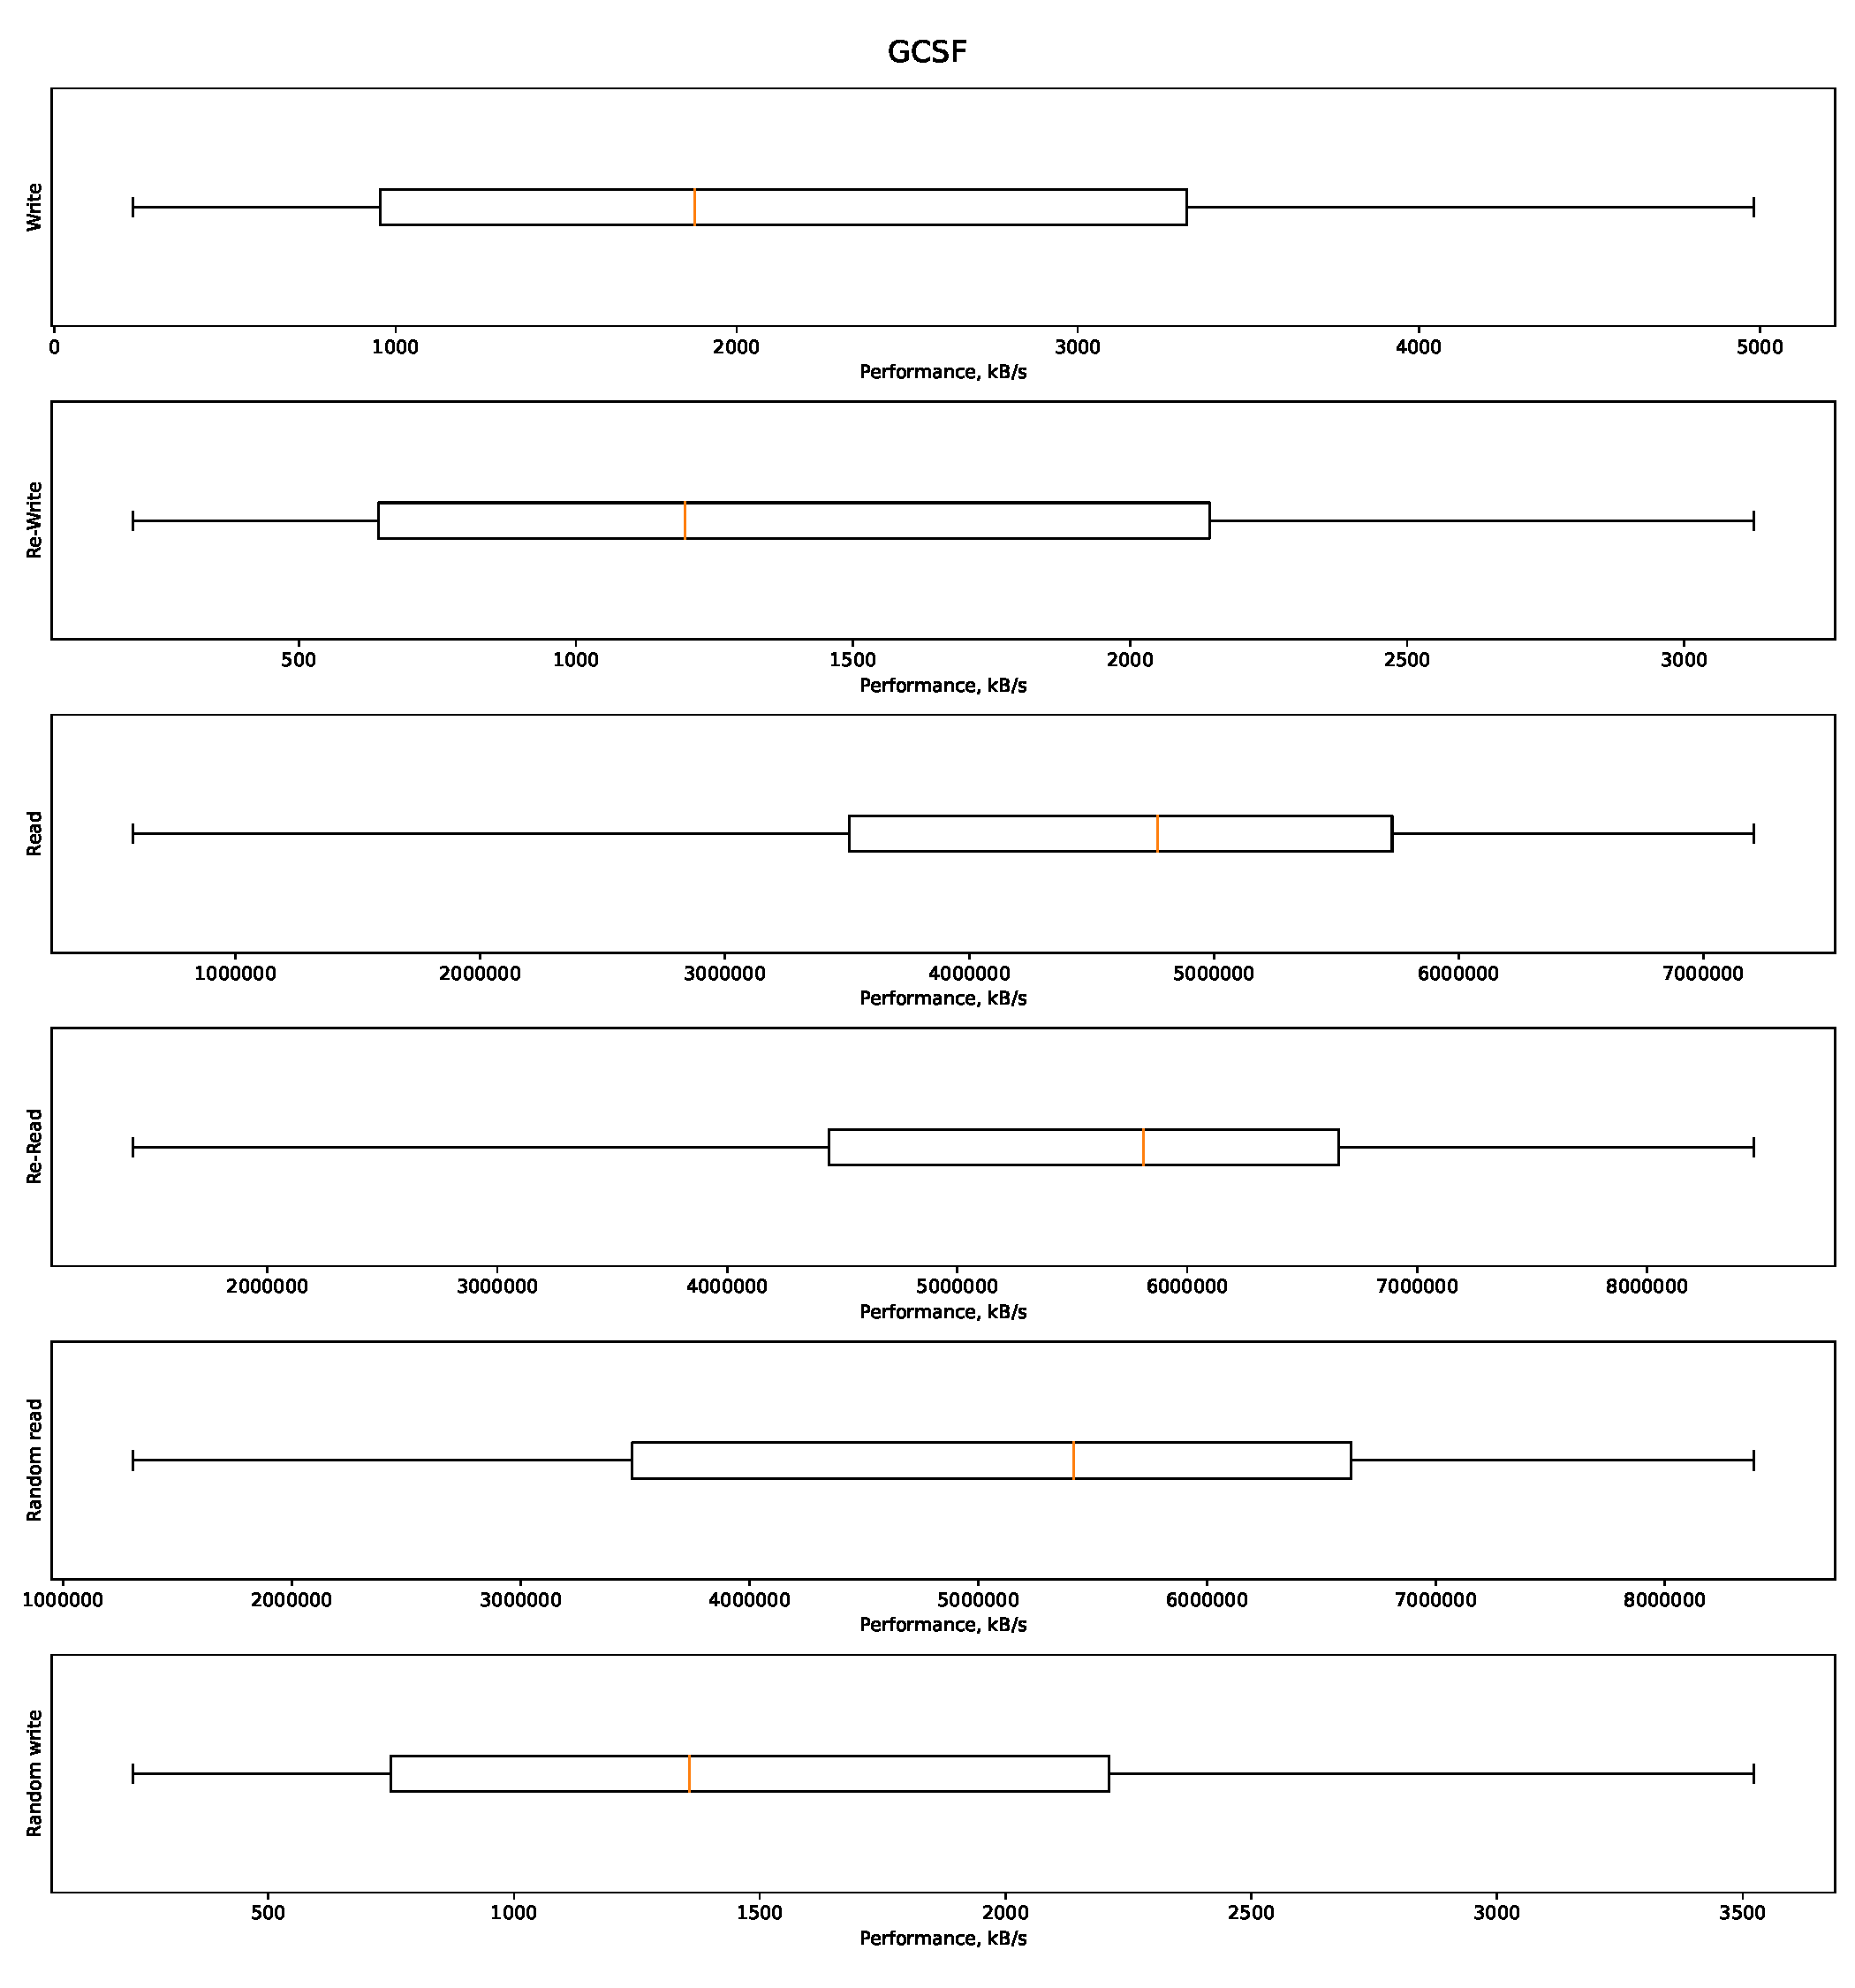
\includegraphics[width=1.0\textwidth]{figures/benchmarking/gcsf/GCSF-box.pdf}
	\end{center}
	\caption{Box plot of the IOZone output for the different tests for GCSF}
\end{figure}

Figure~\ref{fig:res_box_fffs} presents a box plot of the benchmarking results of FFFS. In this plot, it is possible to see tha the spread of the values from Write and Re-Write is high. Looking at Table~\ref{tbl:data_write_fejk_ffs}, we can see that certain values are indeed greater than the most, such as \texttt{file size = 2048, buffer size = 128} where the performance is \SI[per-mode = symbol]{116330}{\kilo\byte\per\second} which is significantly more than most values in the table. Further, Figure~\ref{fig:res_box_fffs} shows that Read, Re-Read and Random Read have similar performances, where the average and best performance of Re-Read and Random Read is better than the average and best performance of Read. Random Write has less of a spread than Write and Re-Write has, and the average performance of Random Write is better than the average performance of both Write and Re-Write.

\begin{figure}[!htb]
	\label{fig:res_box_fffs}
	\begin{center}
		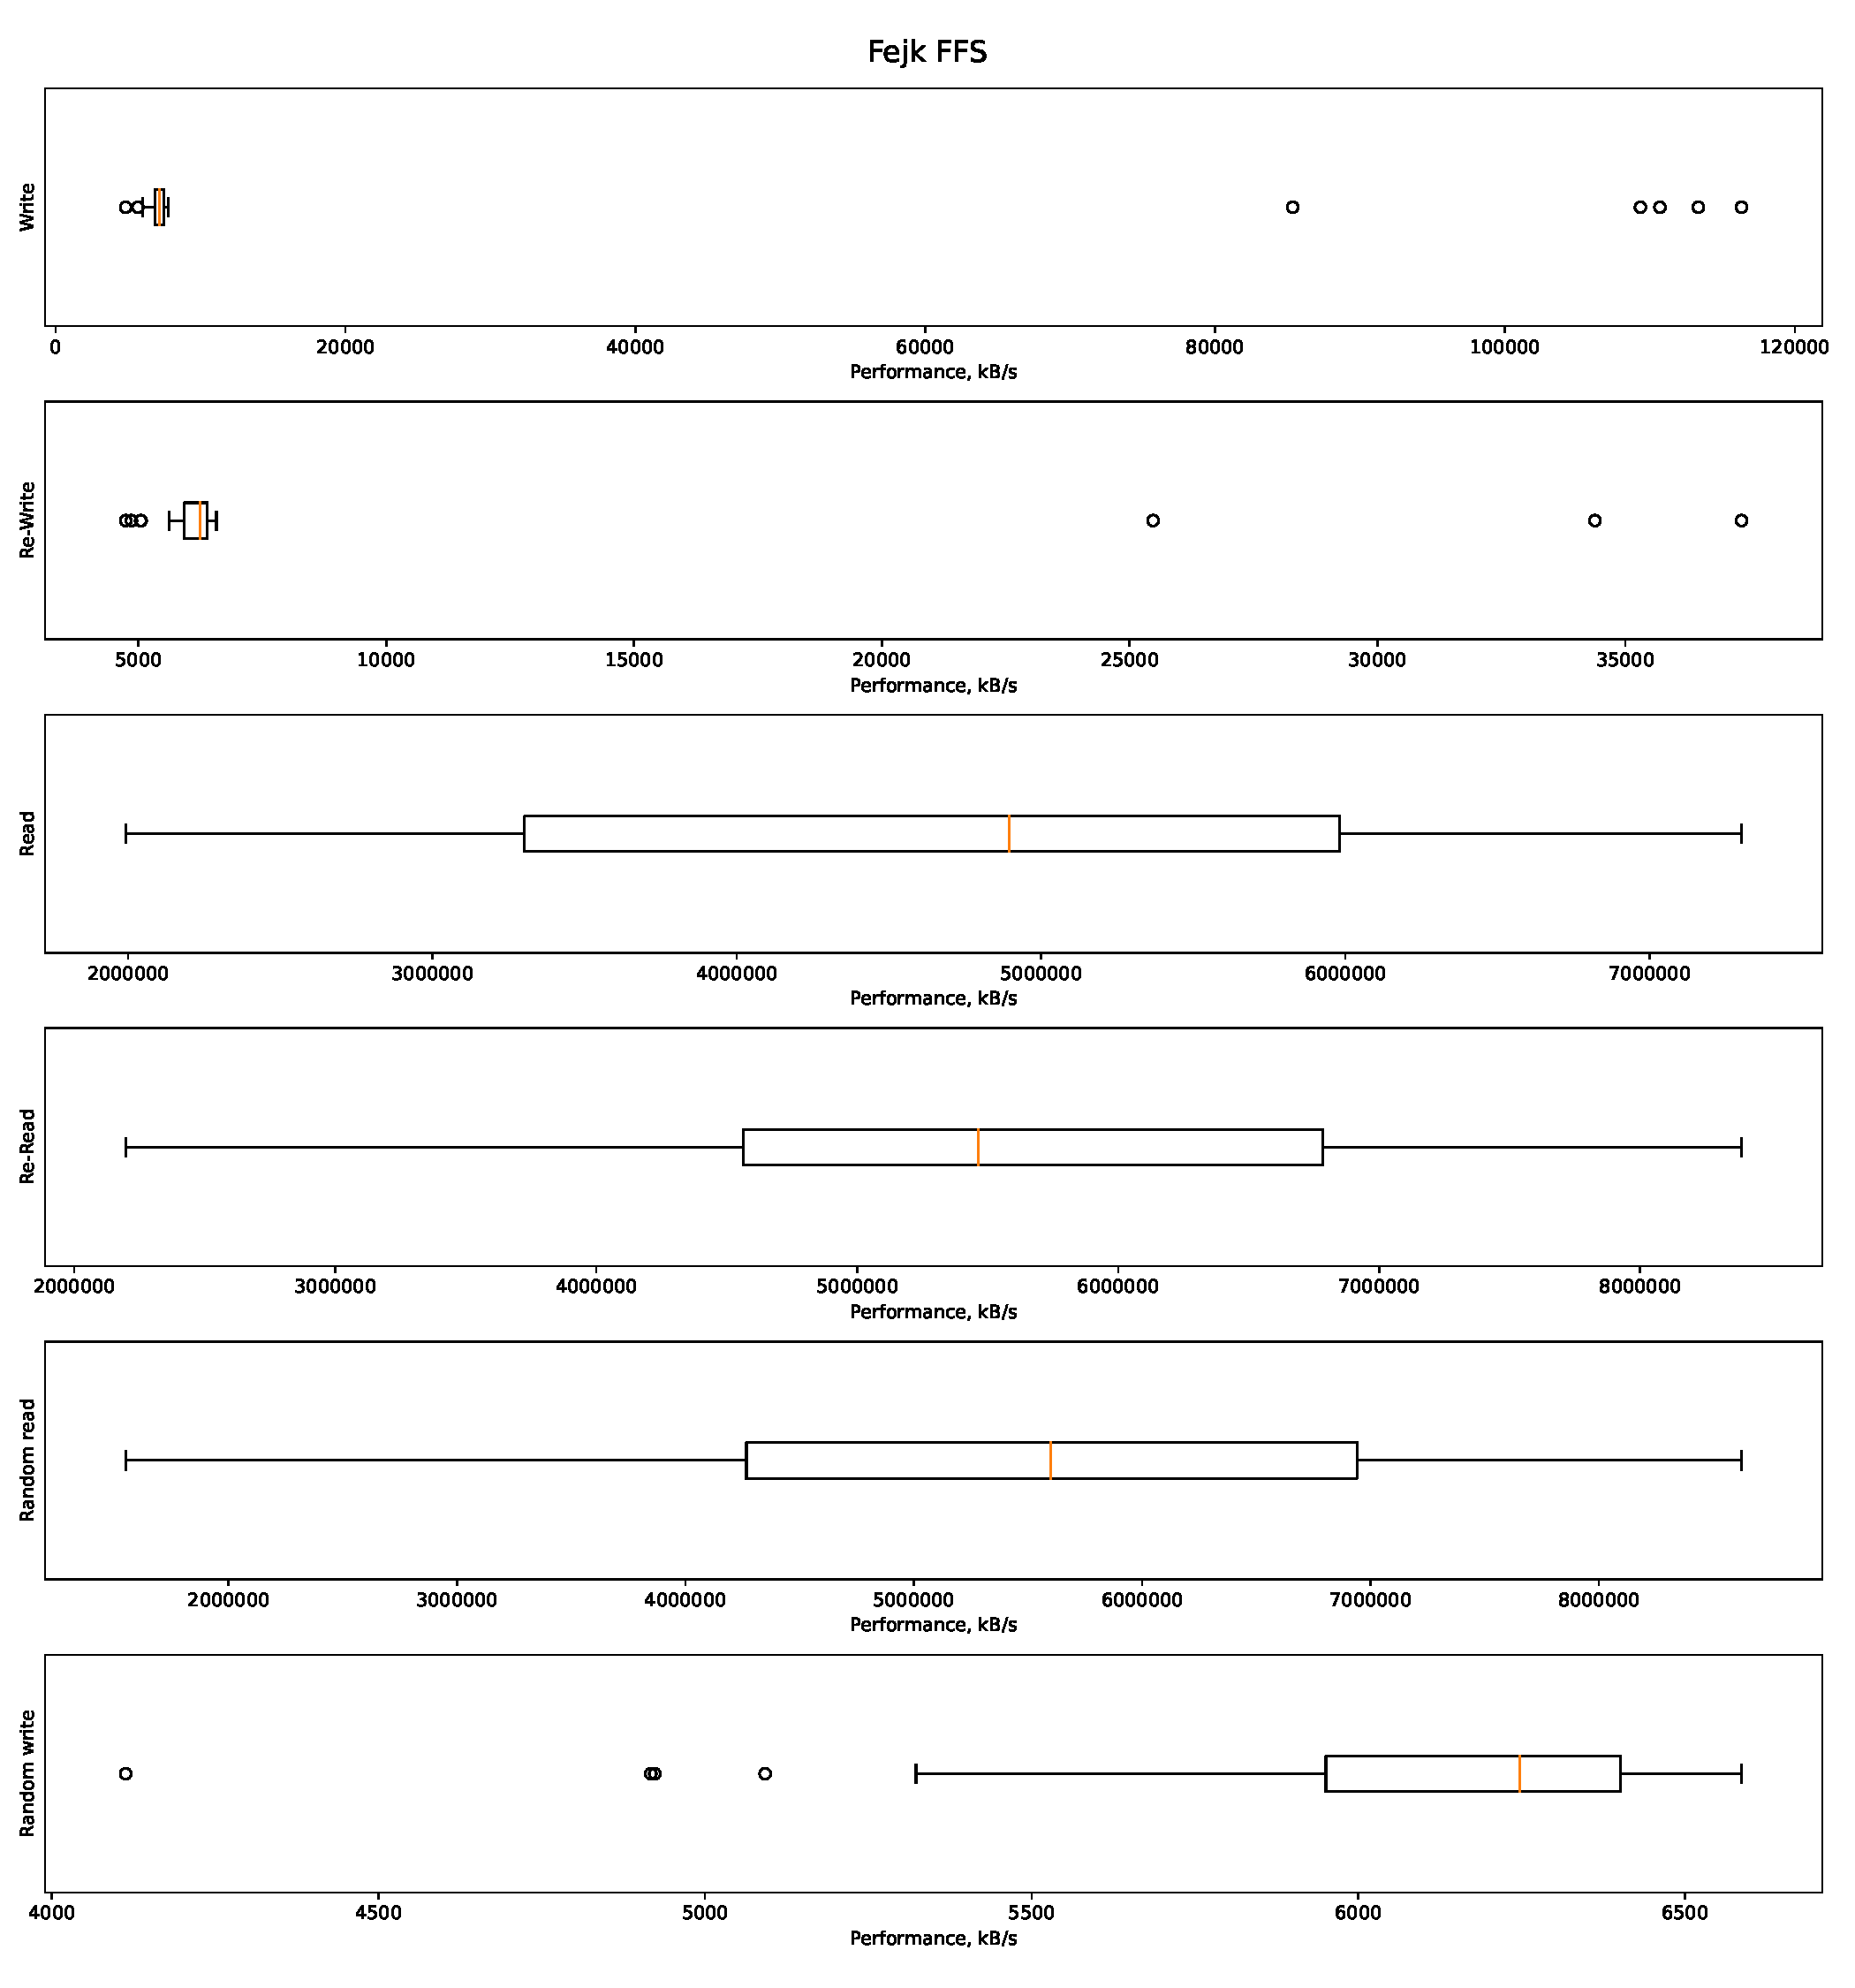
\includegraphics[width=1.0\textwidth]{figures/benchmarking/fake-ffs/Fejk FFS-box.pdf}
	\end{center}
	\caption{Box plot of the IOZone output for the different tests for FFFS}
\end{figure}

Figure~\ref{fig:res_box_apfs} presents a box plot for APFS. In this figure, it is possible to see that the performance of the different write operations are lower than the performance of the read operations. Further, it can be noted that the average performance of the Re-Read and the Re-Write tests are better than the performance of the standard Read and Write tests. The average performance of Random Read is similar to the average performance of Read, but the average performance of Random Write is significantly lower than the average performance of Write.

\begin{figure}[!htb]
	\label{fig:res_box_apfs}
	\begin{center}
		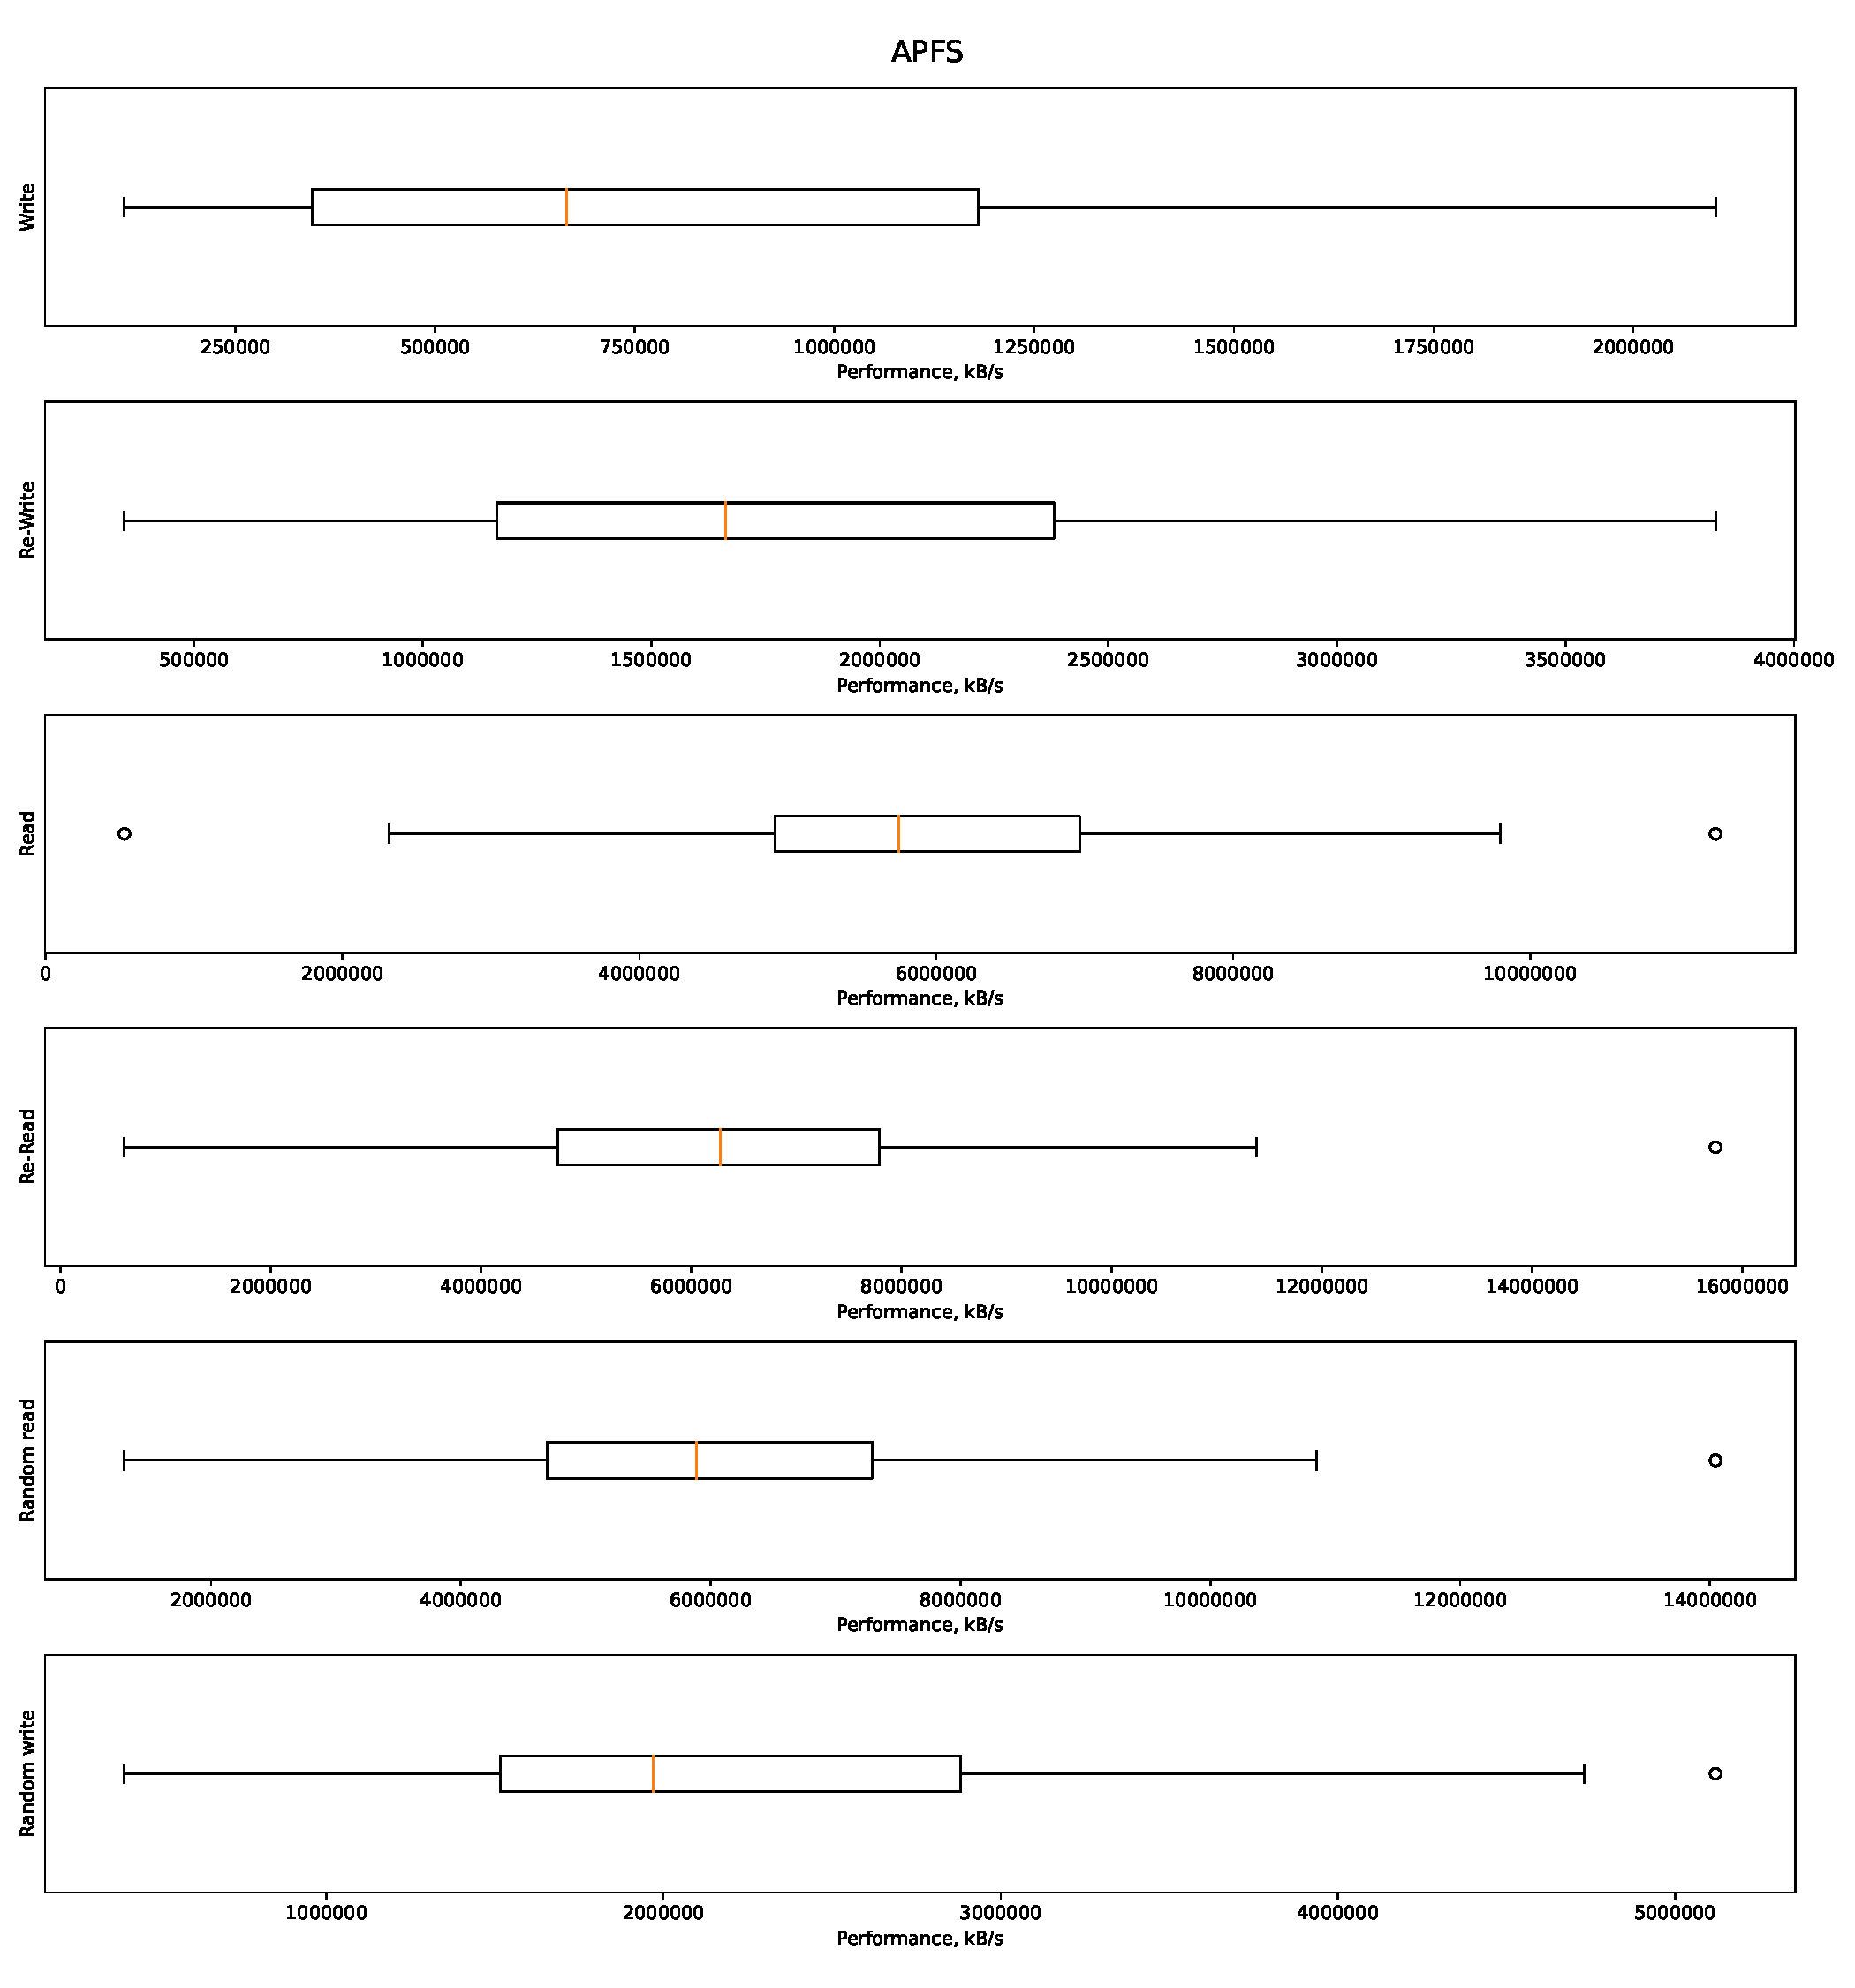
\includegraphics[width=1.0\textwidth]{figures/benchmarking/local/APFS-box.pdf}
	\end{center}
	\caption{Box plot of the IOZone output for the different tests for APFS}
\end{figure}